\documentclass{beamer} 
\usepackage[utf8]{inputenc}
\usepackage[ngerman,english]{babel}
\usepackage{xcolor}
\usepackage{multicol}
 \begin{document}
 	\selectlanguage{ngerman}
 	\title[Crisis]
 	{Entwicklung eines interaktiven Programms zur Simulation und Veranschaulichung von quantenmechanischen Wellenfunktionen}
 	\author % (optional, for multiple authors)
 	{Patrick Richter}
 	\date % (optional)
 	{16.7.2020}
 	
 	\addtobeamertemplate{navigation symbols}{}{ \hspace{1em}    \usebeamerfont{footline}%
 		\insertframenumber / \inserttotalframenumber }
 	\begin{frame}[plain]
 		\titlepage
 	\end{frame}
 \begin{frame}
 	\frametitle{Übersicht}
 	\tableofcontents
 \end{frame}
\section{Die numerische Berechnung der Schrödingergleichung}
 	\begin{frame}
 		\frametitle{Übersicht}
 		\tableofcontents[currentsection]
 	\end{frame}
 	\begin{frame}
 		\frametitle{Die Schrödingergleichung}
 		\begin{equation*}
 			i\hbar\frac{\partial}{\partial t}\Psi(x,t)=- \frac{\hbar^2}{2m}\Delta \Psi(x, t) + V(x, t) \Psi(x, t)
 			\label{Schroedingergleichnung}
 		\end{equation*}
 		%More content goes heredarkgreen
 	\end{frame}
\begin{frame}
\frametitle{Numerische Berechnung}
\begin{figure}
	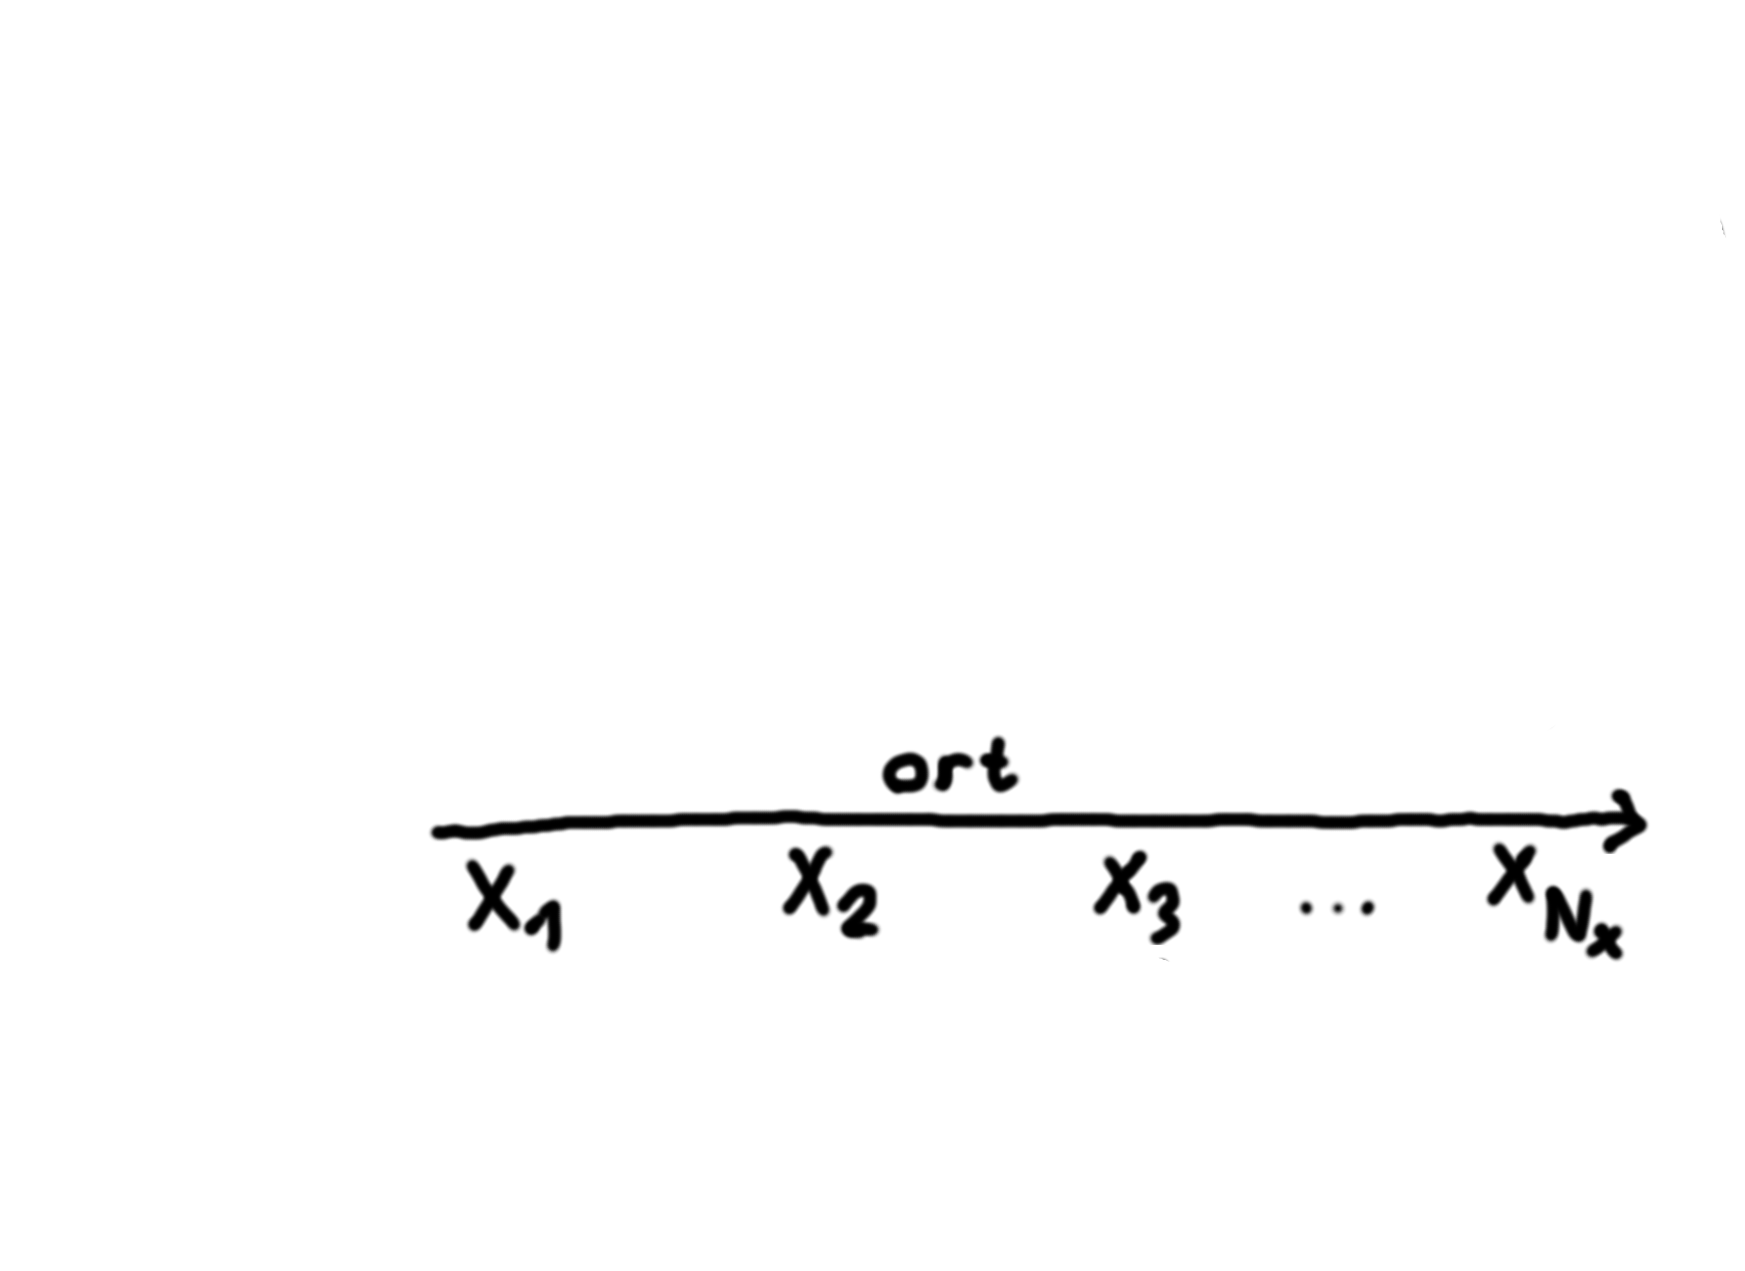
\includegraphics[width=0.8\linewidth,height=\textheight,keepaspectratio]{./numerisch1.png}
\end{figure}
\end{frame}
\begin{frame}
\frametitle{Numerische Berechnung}
\begin{figure}
	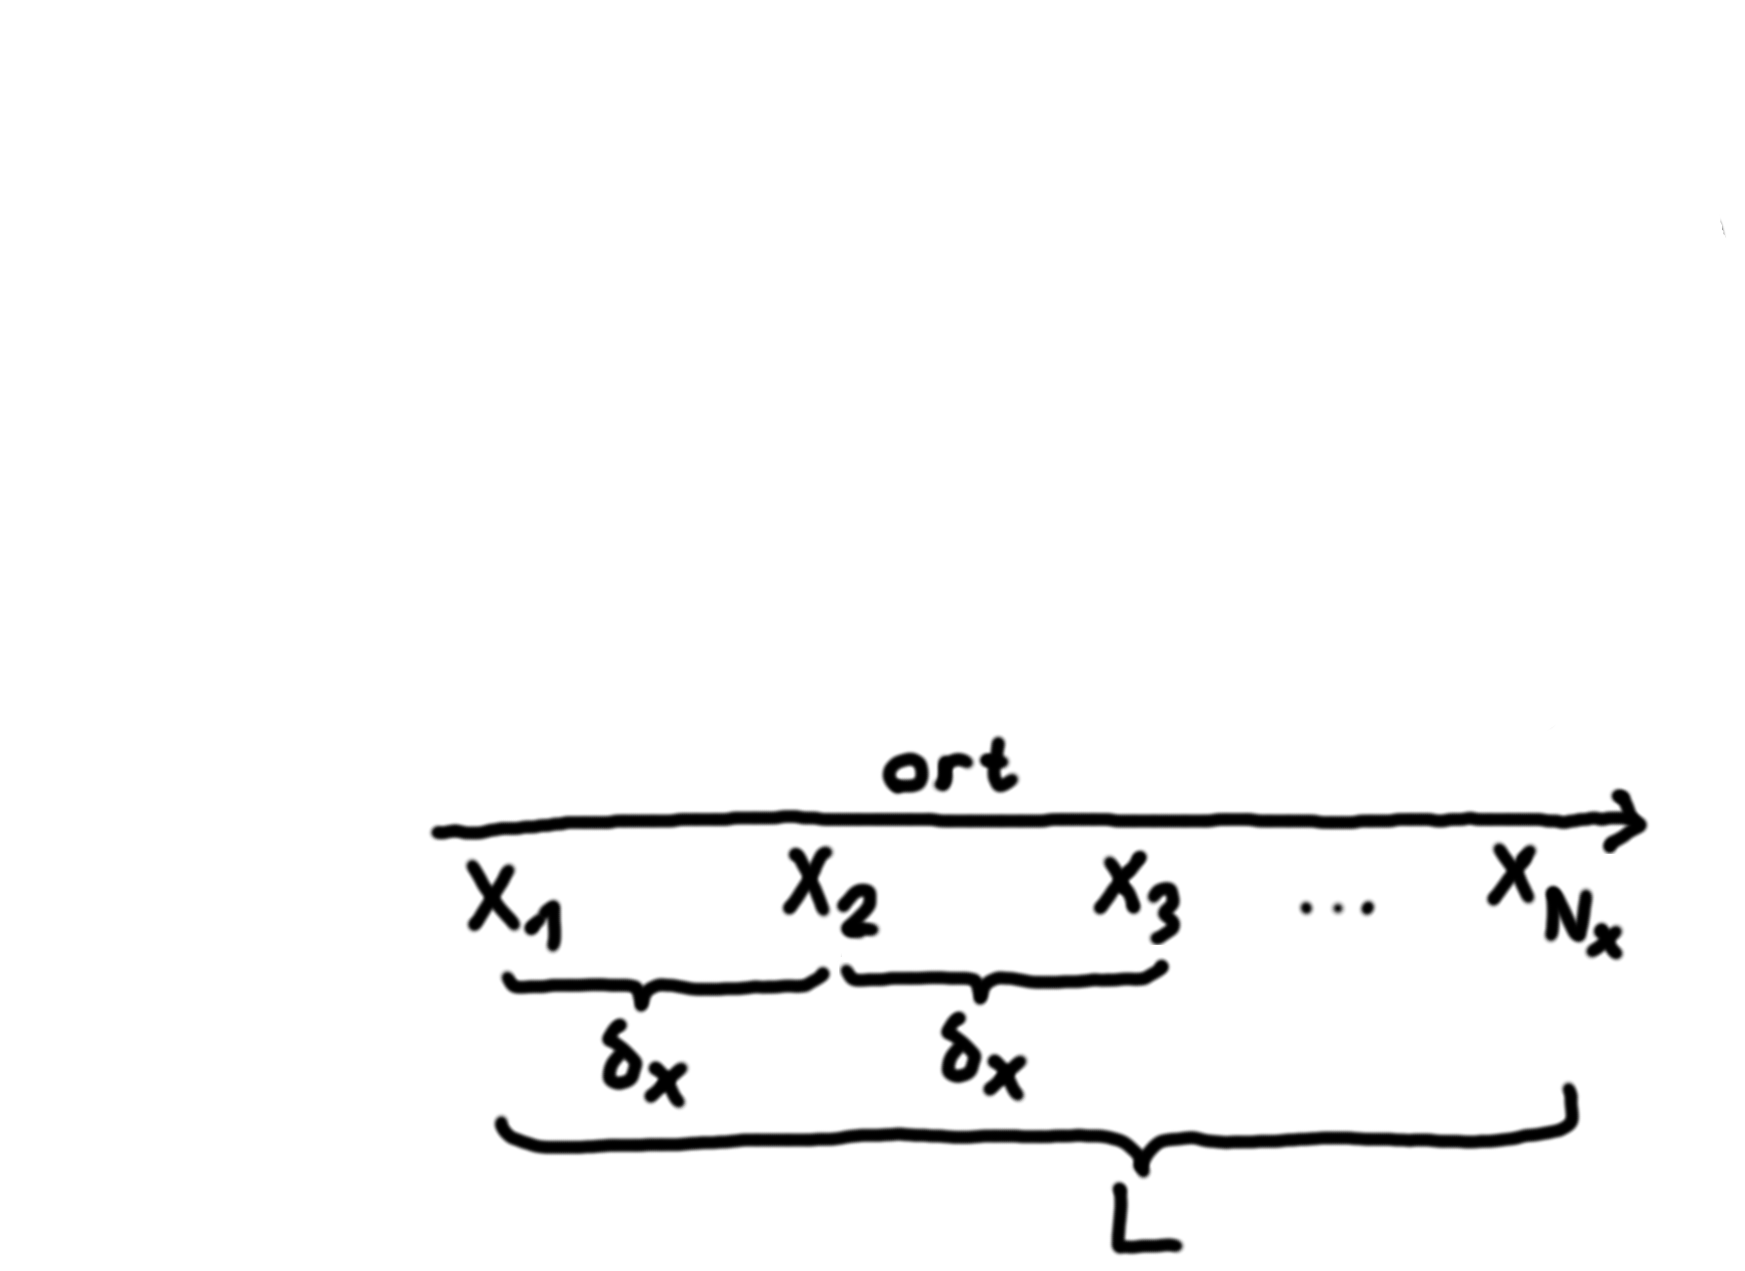
\includegraphics[width=0.8\linewidth,height=\textheight,keepaspectratio]{./numerisch2.png}
\end{figure}
\end{frame}
\begin{frame}
\frametitle{Numerische Berechnung}
\begin{figure}
	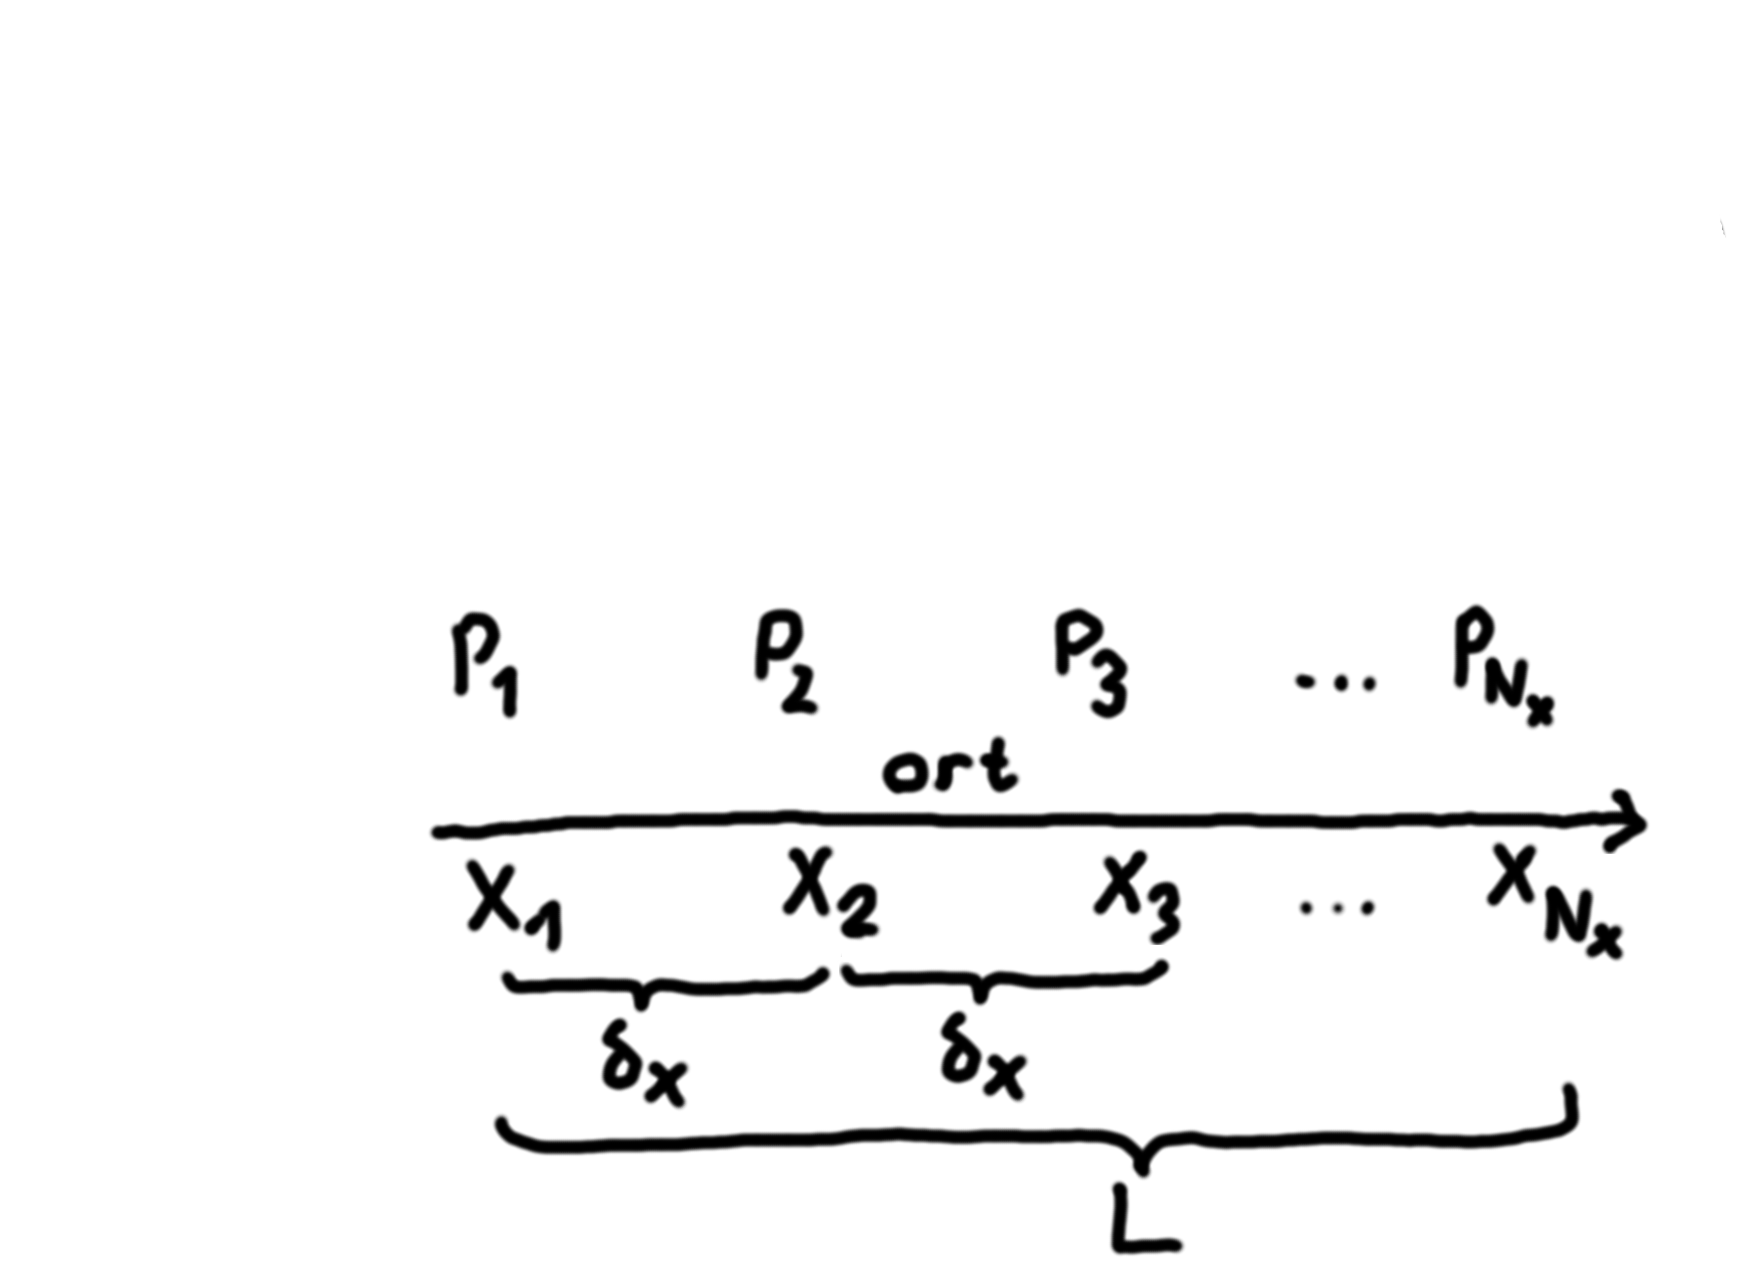
\includegraphics[width=0.8\linewidth,height=\textheight,keepaspectratio]{./numerisch3.png}
\end{figure}
\end{frame}
\begin{frame}
\frametitle{Numerische Berechnung}
\begin{figure}
	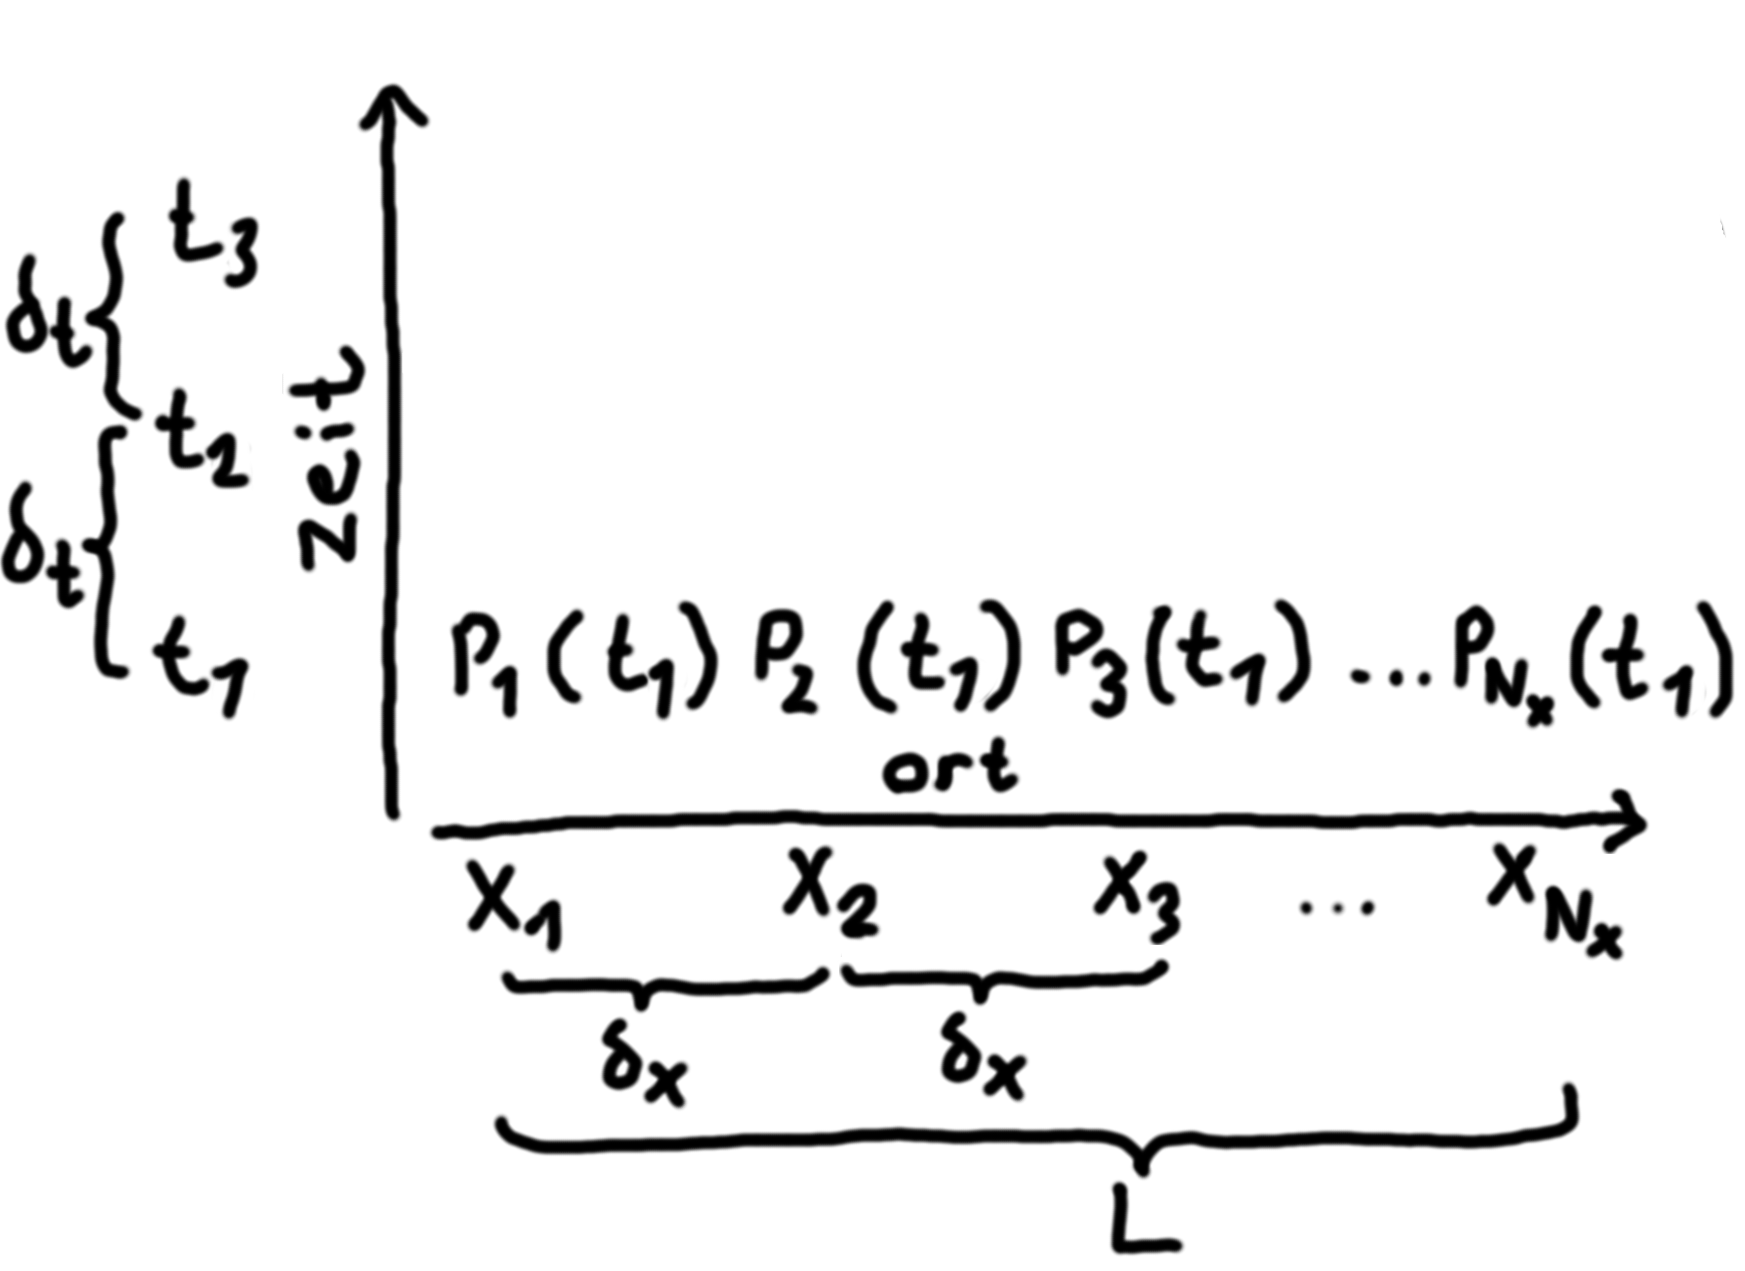
\includegraphics[width=0.8\linewidth,height=\textheight,keepaspectratio]{./numerisch4.png}
\end{figure}
\end{frame}
\begin{frame}
\frametitle{Numerische Berechnung}
\begin{figure}
	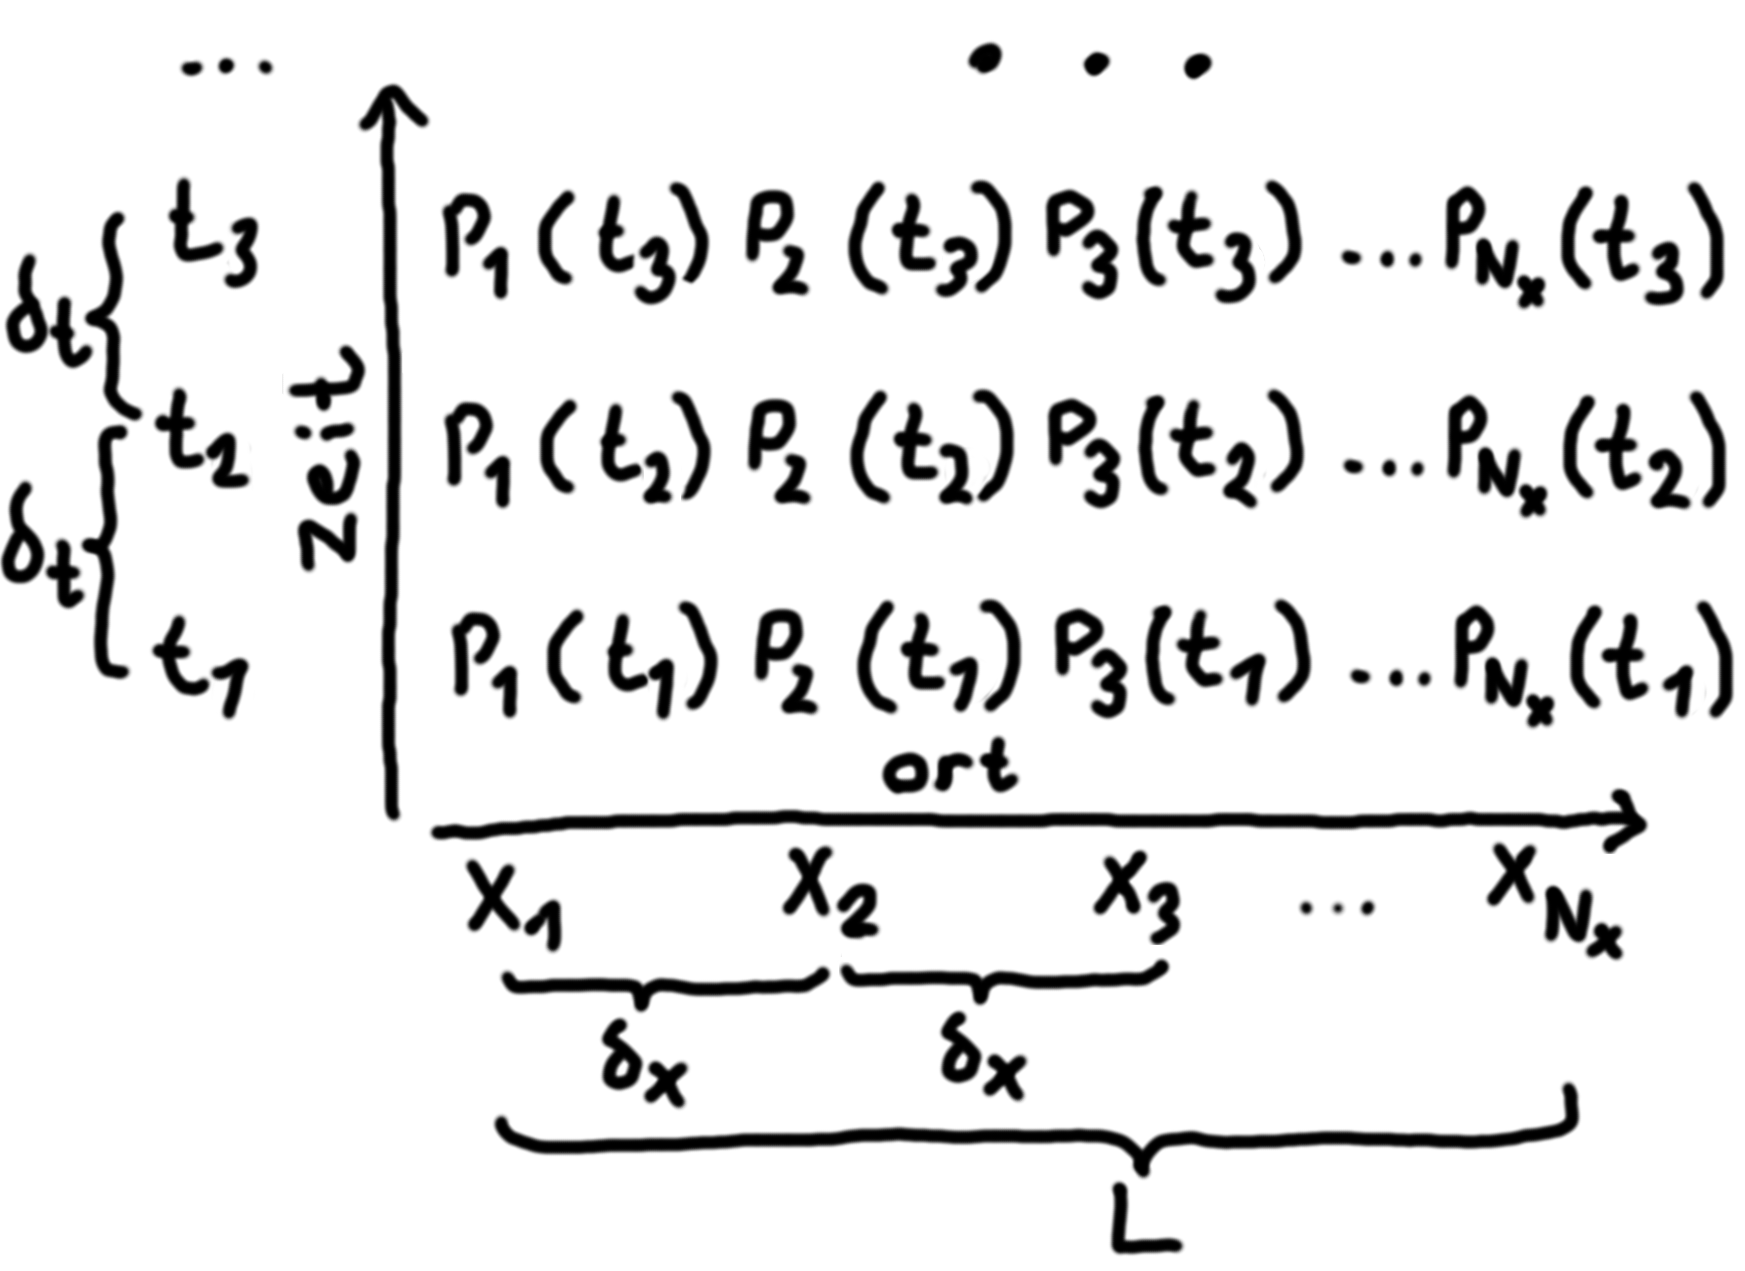
\includegraphics[width=0.8\linewidth,height=\textheight,keepaspectratio]{./numerisch5.png}
\end{figure}
\end{frame}
\begin{frame}
\frametitle{Die Schrödingergleichung}
\begin{equation*}
i\hbar\frac{\partial}{\partial t}\Psi(x,t)=- \frac{\hbar^2}{2m}\Delta \Psi(x, t) + V(x, t) \Psi(x, t)
\label{Schroedingergleichnung}
\end{equation*}
%More content goes here
\end{frame}
 \begin{frame}
	 \frametitle{Die Finite-Differenzen-Methode}
	 \begin{equation*}
	 	\big[\Delta\Psi(x, t)\big]_{x = x_n}=\frac{p_{n-1} + p_{n + 1} - 2 p_n}{(\delta_x)^2}
	 \end{equation*}
	 %More content goes here

\end{frame}
\begin{frame}
	\frametitle{Die numerische Zeitableitung}
	\begin{equation*}
	f(\Psi, t):=\frac{\partial \Psi}{\partial t}
	\end{equation*}
	\pause
	\begin{equation*}
	\frac{\partial}{\partial t}\Psi(x,t) = \frac{i\hbar}{2m}\Delta \Psi(x, t) - \frac{i}{\hbar} V(x, t) \Psi(x, t)
	\end{equation*}
\end{frame}
\begin{frame}
\frametitle{Das explizite Runge-Kutta-Verfahren}
{\begin{equation*}
\Psi_{t + \delta_t} = \Psi_t + \delta_t \sum_{j = 1}^{R} b_j \Omega_j
\end{equation*}
\begin{equation*}
\Omega_j = f(\Psi_t + \delta_t\sum_{l = 1}^{j - 1}a_{jl}\Omega_l, t + c_j \delta_t)
\end{equation*}}
\\
\textcolor{brown}{
	\(R\): Ordnung\\
	\(a_{j l}\),\(b_j\), \(c_j\): Koeffizienten
}
\begin{multicols}{2}
	\pause
	\begin{equation*}
	\begin{array}{ccccc|c}
	& 		&  		&  		&  		& c_1\\
	a_{2,1} & 		&  		&  		&  		& c_2\\
	a_{3,1} &a_{3,2}& 		&  		&  		& c_3\\
	\vdots 	&\vdots	&\ddots	&  		&  		& \vdots\\
	a_{R,1}	&a_{R,2}&\dots	&a_{R,R-1}&  	& c_R\\
	\hline  
	b_1    & b_2   	& \dots &b_{R-1}& b_R	&\\
	\end{array}\; 
	\label{runge_tabelle}
	\end{equation*}
	\pause
	\begin{equation*}
	\label{runge_tabelle}
	\begin{array}{cccc|c}
	& 		&  		&  		& 0\\
	\frac{1}{2} & 	& 		&  		& \frac{1}{2}\\
	0 	& \frac{1}{2}	&  & & \frac{1}{2}\\
	0& 0	& 1 & & 1\\
	\hline  
	\frac{1}{6}    	& \frac{1}{3}  	& \frac{1}{3} & \frac{1}{6} 	& \\
	\end{array}
	\end{equation*}
\end{multicols}
%More content goes here


\end{frame}
\section{Überprüfung der numerischen Simulationsergebnisse}
\begin{frame}
\frametitle{Übersicht}
\tableofcontents[currentsection]
\end{frame}
\begin{frame}
	\frametitle{Der unendlich hohe Potentialkasten}
	\begin{equation*}
		\Psi_k(x, t)\big|_{[0, L]} = \sin(A x) e^{i B t}  C
	\end{equation*}
	\textcolor{brown}{
		\begin{multicols}{3}
			\noindent
			\begin{equation*}
			A(k) = \frac{k \pi}{L}
			\end{equation*}
			\begin{equation*}
			B(k) = -\frac{\hbar}{2m}\bigg(\frac{k \pi}{L}\bigg)^2
			\end{equation*}
			\begin{equation*}
			C = \sqrt{\frac{2}{L}}
			\end{equation*}
		\end{multicols}
	}
\pause
	\begin{equation*}
	\Psi_\text{a}(x, t) = \sum_{k = 1}^{Q}c_k \Psi_k(x, t)
	\end{equation*}
	\textcolor{brown}{
		\begin{equation*}
		\sum_{k = 1}^{Q}|c_k|^2 = 1
		\end{equation*}
	}
\end{frame}
\begin{frame}
\frametitle{Definition des Fehlerkriteriums \(\Theta\)}
\begin{equation}
D(x_n, t) = |p_n(t) - \Psi_\text{a}(x_n, t)|
\end{equation}
\pause
\begin{equation}
\theta(t) = \int_{\text{num}}D(x, t)dx
\label{durchschnittsabweichung}
\end{equation}
\pause
\begin{equation}
\Theta(t) = \frac{\theta(t)}{\int_\text{num} |\Psi_\text{a}(x, t)|dx}
\end{equation}

\end{frame}
\begin{frame}
	\frametitle{Der Zeitverlauf des Fehlers im numerisch stabilen Fall}	
\begin{figure}
	\includegraphics[width=0.8\linewidth,height=\textheight,keepaspectratio]{../plots/zeitentwicklung/uebersicht/uebersicht.pdf}
	\label{konvergenzzeitentwicklung}
\end{figure}
\textcolor{brown}{
\(L = 1000\)\hspace{3em} \( \delta_t, \delta_x, m = 1\)\hspace{3em} \(Q = 50\)
}
\end{frame}
\begin{frame}
\frametitle{Der Zeitverlauf des Fehlers im numerisch instabilen Fall}
\begin{figure}
	\includegraphics[width=0.8\linewidth,height=\textheight,keepaspectratio]{../plots/divergenz/divergenz.pdf}
	\label{divergenzzeitentwicklung}
\end{figure}
\textcolor{brown}{
\(L = 1000\)\hspace{3em} \(\delta_x, m = 1\)\hspace{3em} \(Q = 50\)
}
\end{frame}
\begin{frame}
	\frametitle{Simulation über das Zeitintervall \(T\) in \(Z\) Zeitschritten}
	\begin{equation*}
		\delta_t = \frac{T}{Z}
	\end{equation*}
\end{frame}
\begin{frame}
\frametitle{Der Fehler in Abhängigkeit von \(\delta_x\)}
\begin{figure}
	\includegraphics[width=0.8\linewidth,height=\textheight,keepaspectratio]{../plots/raumUndZeitpunkte/deltaxExtrem/plot.pdf}
	\label{deltaxthetafit}
\end{figure}
\textcolor{brown}{
\(L,T = 1000\)\hspace{3em} \(m = 1\)\hspace{3em}\(Z = 10000\)\hspace{3em}\(\delta_t = 0.1\)\hspace{3em} \(Q = 50\)
}
\end{frame}
\begin{frame}
\frametitle{Der Fehler in Abhängigkeit von \(\delta_t\)}
\begin{figure}
	\includegraphics[width=0.8\linewidth,height=\textheight,keepaspectratio]{../plots/raumUndZeitpunkte/deltat/zoom/deltat.pdf}
	\label{deltatthetanah}
\end{figure}
\textcolor{brown}{
\(L,T, N_x = 1000\)\hspace{3em} \(m = 1\)\hspace{3em}\(\delta_x = \frac{1000}{999}\)\hspace{3em} \(Q = 50\)
}
\end{frame}
\begin{frame}
\frametitle{Der Fehler in Abhängigkeit von \(\delta_t\) für verschiedene \(N_x\)}
\begin{figure}
	\includegraphics[width=0.8\linewidth,height=\textheight,keepaspectratio]{../plots/raumUndZeitpunkte/deltat/deltat.pdf}
	\label{deltattheta}
\end{figure}
\textcolor{brown}{
\(L,T = 1000\)\hspace{3em} \(m = 1\)\hspace{3em} \(Q = 50\)
}
\end{frame}
\begin{frame}
\frametitle{Die kritischen \(\delta_x\) in Abhängigkeit von \(\delta_t\)}
\begin{figure}
	\includegraphics[width=0.8\linewidth,height=\textheight,keepaspectratio]{../plots/raumUndZeitpunkte/optimum/optimum.pdf}
	\label{deltathetaxmin}
\end{figure}
\textcolor{brown}{
\(L,T = 1000\)\hspace{3em} \(m = 1\)\hspace{3em} \(Q = 50\)
}
\end{frame}
\begin{frame}
\frametitle{Fehler und Norm in Abhängigkeit der Ordnung}

\begin{figure}
	\includegraphics[width=0.8\linewidth,height=\textheight,keepaspectratio]{../plots/ordnung/mitBetrag/ordnung.pdf}
	\label{ordnunguebersicht}
\end{figure}
\textcolor{brown}{
\(L, T = 1000\)\hspace{3em} \( \delta_t, \delta_x, m = 1\)}
\end{frame}
\section{Das Programm}
\begin{frame}
\frametitle{Übersicht}
\tableofcontents[currentsection]
\end{frame}
\begin{frame}
\frametitle{Das Programm}
\textcolor{blue}{
\href{https://quantsimulant.de/versionen/bachelorarbeit}{https://quantsimulant.de/versionen/bachelorarbeit}
}
\end{frame}
\begin{frame}
\frametitle{Die Bachelorarbeit}
\textcolor{blue}{
	\href{https://quantsimulant.de/versionen/bachelorarbeit/arbeit.pdf}{https://quantsimulant.de/versionen/bachelorarbeit/arbeit.pdf}
}
\end{frame}
 	% etc
 \end{document}
